% Slide bảo vệ giữa kỳ, bản chung của nhóm.
% Biên dịch bằng XeLaTeX (Overleaf: Menu > Compiler > XeLaTeX).
\documentclass[aspectratio=169,11pt]{beamer}

\usepackage{fontspec}
\setmainfont{texgyreheros}[Extension=.otf,UprightFont=*-regular,BoldFont=*-bold,ItalicFont=*-italic,BoldItalicFont=*-bolditalic]
\setsansfont{texgyreheros}[Extension=.otf,UprightFont=*-regular,BoldFont=*-bold,ItalicFont=*-italic,BoldItalicFont=*-bolditalic]
\setmonofont{texgyrecursor}[Extension=.otf,UprightFont=*-regular,BoldFont=*-bold,ItalicFont=*-italic,BoldItalicFont=*-bolditalic]
\usepackage[vietnamese]{babel}
\usepackage{tikz}
\usetikzlibrary{arrows.meta,positioning,calc}
\usepackage{tabularx}
\usepackage{booktabs}
\usepackage{colortbl}
\usepackage{array}

% ---- Màu: xanh tableheader của báo cáo làm màu nhấn ----
\definecolor{accent}{RGB}{68,114,196}
\definecolor{accentlight}{RGB}{234,240,250}
\definecolor{accentdark}{RGB}{38,62,110}
\definecolor{ink}{RGB}{38,42,52}
\definecolor{muted}{RGB}{110,116,128}
\definecolor{warn}{RGB}{196,80,90}

\setbeamercolor{normal text}{fg=ink,bg=white}
\setbeamercolor{structure}{fg=accent}
\setbeamercolor{frametitle}{fg=accentdark,bg=white}
\setbeamercolor{itemize item}{fg=accent}
\setbeamercolor{itemize subitem}{fg=accent}
\setbeamercolor{block title}{fg=white,bg=accent}
\setbeamercolor{block body}{fg=ink,bg=accentlight}
\setbeamertemplate{navigation symbols}{}
\setbeamertemplate{itemize item}[square]
\setbeamertemplate{itemize subitem}[circle]
\setbeamerfont{itemize/enumerate body}{size=\normalsize}
\setbeamerfont{itemize/enumerate subbody}{size=\small}
\setbeamertemplate{blocks}[rounded][shadow=false]

% Tiêu đề khung: chữ đậm xanh đậm + vạch xanh
\setbeamertemplate{frametitle}{%
  \vskip 3mm
  \usebeamercolor[fg]{frametitle}\usebeamerfont{frametitle}\bfseries\Large\insertframetitle\par
  \vskip 1.2mm
  {\color{accent}\hrule height 1.2pt}
}
% Chân trang: tên + số trang
\setbeamertemplate{footline}{%
  \hbox to \paperwidth{%
    \hspace{8mm}\color{muted}\scriptsize Phát hiện biển số xe và tách ký tự bằng xử lý ảnh cổ điển%
    \hfill\insertframenumber\,/\,\inserttotalframenumber\hspace{8mm}}
  \vskip 4mm}
\setbeamersize{text margin left=9mm,text margin right=9mm}

\newcommand{\code}[1]{{\footnotesize\ttfamily #1}}
\newcommand{\acc}[1]{\textcolor{accent}{\textbf{#1}}}
\newcommand{\hl}[1]{\textcolor{accentdark}{\textbf{#1}}}

\renewcommand{\arraystretch}{1.18}
\newcommand{\barrow}[4]{%
  \node[anchor=east,align=right] at (-1.5,#1) {#2};
  \fill[accent] (0,#1-0.26) rectangle (#3,#1+0.26);
  \node[anchor=west] at (#3+1.5,#1) {#4};}
\newcommand{\hd}[1]{\cellcolor{accent}\textcolor{white}{\bfseries #1}}
\newcolumntype{C}{>{\centering\arraybackslash}X}
\newcolumntype{Y}{>{\raggedright\arraybackslash}X}

\title{Phát hiện biển số xe và tách ký tự\\bằng xử lý ảnh cổ điển}
\subtitle{Báo cáo giữa kỳ}
\author{Bùi Thuỳ Châu Anh (24001963)\and Nguyễn Ngọc Bích (24001977)}
\date{MAT3562E Computer Vision, HK1 2026--2027}

\begin{document}

% ============ Tiêu đề ============
\begin{frame}[plain]
  \begin{tikzpicture}[remember picture,overlay]
    \fill[accent] (current page.north west) rectangle ([yshift=-4.2cm]current page.north east);
    \node[anchor=north west,xshift=9mm,yshift=-7mm,text=white,align=left] at (current page.north west)
      {\fontsize{9}{11}\selectfont\bfseries TRƯỜNG ĐẠI HỌC KHOA HỌC TỰ NHIÊN, ĐHQGHN};
    \node[anchor=north east,xshift=-9mm,yshift=-5mm,fill=white,rounded corners=3pt,inner sep=2.5mm] at (current page.north east)
      {
\includegraphics[height=2.3cm]{figures/HUS.png}};
    \node[anchor=south west,xshift=9mm,yshift=-4.2cm+4mm,text=white,align=left,text width=0.72\paperwidth] at (current page.north west)
      {\fontsize{22}{26}\selectfont\bfseries Phát hiện biển số xe và tách ký tự bằng xử lý ảnh cổ điển};
  \end{tikzpicture}
  \vspace{3.55cm}
  \begin{flushleft}
    {\large\bfseries\color{accentdark} Báo cáo giữa kỳ}\\[1mm]
    {\color{muted}Bài toán, phương pháp, kết quả thí nghiệm và phân tích lỗi}\\[5mm]
    \small
    \begin{tabular}{@{}l@{\hspace{6mm}}l@{}}
      \hl{Nhóm thực hiện} & Bùi Thuỳ Châu Anh (24001963), Nguyễn Ngọc Bích (24001977)\\
      \hl{Môn học} & MAT3562E Computer Vision, HK1 2026--2027\\
      \hl{Giảng viên} & TS. Cao Văn Chung\\
    \end{tabular}
  \end{flushleft}
\end{frame}

% ============ Bài toán + dữ liệu ============
\begin{frame}{Bài toán và dữ liệu}
  \begin{columns}[T]
    \column{0.50\textwidth}
    \begin{itemize}
      \item Kịch bản: camera cố định ở bãi gửi xe, mỗi ảnh có đúng một biển.
      \item Đầu ra giữa kỳ: hộp biển, ảnh biển đã nắn, danh sách hộp ký tự.
      \item Chỉ dùng \hl{xử lý ảnh cổ điển}, không học sâu.
      \item Dữ liệu: tập con CCPD2019, 660 ảnh biển xanh 7 ký tự: \code{base} 500 và bốn nhóm khó (\code{tilt}, \code{blur}, \code{db}, \code{challenge}) mỗi nhóm 40.
      \item Chọn tham số trên \acc{tune} (30\%), chỉ báo cáo trên \acc{test} (70\%).
    \end{itemize}
    \column{0.48\textwidth}
    \vspace{2mm}
    \small
    \begin{tabularx}{\linewidth}{>{\raggedright\arraybackslash}Xrr}
      \rowcolor{accent}\hd{Nhóm} & \hd{tune} & \hd{test}\\
      base & 150 & 350\\
      \rowcolor{accentlight}mỗi nhóm khó & 12 & 28\\
      \textbf{Tổng} & \textbf{198} & \textbf{462}\\
    \end{tabularx}
    \vspace{4mm}

    \begin{block}{Độ đo}
      \small
      IoU $\ge 0.5$ với bbox thật; P, R, F1 theo top-1; Recall@$k$ (R@5 là trần của bước xếp hạng).
    \end{block}
  \end{columns}
\end{frame}

% ============ Pipeline ============
\begin{frame}{Tổng quan pipeline}
  \centering
  \vspace{1mm}
  \begin{tikzpicture}[
    node distance=8mm and 5mm,
    boxA/.style={draw=accent,fill=accentlight,thick,rounded corners=3pt,align=center,minimum height=19mm,text width=27mm,font=\footnotesize},
    arr/.style={-{Stealth[length=2.4mm]},thick,color=accentdark}]
    \node[boxA] (in) {Ảnh xe (BGR)};
    \node[boxA,right=of in] (pre) {\textbf{Tiền xử lý}\\resize 800, xám,\\CLAHE, lọc nhiễu};
    \node[boxA,right=of pre] (edge) {\textbf{Định vị theo cạnh}\\Sobel-x, Otsu,\\morph đa tỉ lệ,\\lọc, NMS};
    \node[boxA,right=of edge] (svm) {\textbf{HOG + SVM}\\xếp lại top-5,\\chọn top-1 (bbox)};
    \node[boxA,below=of svm] (quad) {\textbf{Ước lượng quad}\\từ mặt nạ xanh\\(HSV)};
    \node[boxA,left=of quad] (warp) {\textbf{Nắn phối cảnh}\\homography về\\ảnh $220\times 70$};
    \node[boxA,left=of warp] (bin) {\textbf{Nhị phân hóa}\\Otsu / adaptive};
    \node[boxA,left=of bin] (seg) {\textbf{Tách ký tự}\\CCA / projection\\$\to$ hộp ký tự\\trái $\to$ phải};
    \draw[arr] (in)--(pre); \draw[arr] (pre)--(edge); \draw[arr] (edge)--(svm);
    \draw[arr] (svm)--(quad); \draw[arr] (quad)--(warp); \draw[arr] (warp)--(bin); \draw[arr] (bin)--(seg);
  \end{tikzpicture}
\end{frame}

% ============ Thí nghiệm + độ đo ============
\begin{frame}{Các thí nghiệm và cách đo}
  \setbeamerfont{itemize/enumerate body}{size=\small}
  \begin{columns}[T]
    \column{0.47\textwidth}
    \small
    \begin{tabular}{@{}lp{0.72\linewidth}@{}}
      \acc{E0} & khung \code{run\_all}\\
      \acc{E1} & phân tích hệ màu\\
      \acc{E2} & bộ lọc nhiễu\\
      \acc{E3} & HOG + SVM xếp lại ứng viên\\
      \acc{E4} & cắt bbox hay nắn quad\\
      \acc{E5} & nhị phân hóa: Otsu, adaptive\\
      \acc{E6} & tách ký tự: CCA, projection\\
      \acc{E7} & thời gian chạy từng bước\\
      \acc{E8} & biển số Việt Nam (187 ảnh, 139 có bbox), định tính\\
      \acc{Công cụ} & gán nhãn ký tự (\code{label\_chars})\\
    \end{tabular}
    \column{0.50\textwidth}
    \begin{block}{Độ đo tách ký tự}
      \small
      \code{count\_match}: đủ 7 hộp.\\
      \code{pos0}, \code{pos1-6}: hộp trúng khuôn vị trí.\\
      \code{all\_correct}: đủ 7 hộp \emph{và} cả 7 vị trí trúng.
    \end{block}
    \begin{itemize}
      \item Khuôn 7 vị trí chuẩn của biển $440\times140$ mm, quy về ảnh $220\times70$.
      \item Crop \code{gt} (quad thật): đo riêng bộ tách. Crop \code{pred}: cả pipeline.
    \end{itemize}
  \end{columns}
\end{frame}

% ============ Tiền xử lý + E2 ============
\begin{frame}{Tiền xử lý và thí nghiệm E2: bộ lọc nhiễu}
  \begin{columns}[T]
    \column{0.42\textwidth}
    \begin{itemize}
      \item Resize về rộng \acc{800} px (thử 640/720/800 trên tune, 800 tốt nhất), ảnh xám.
      \item CLAHE (clip 2.0, lưới $8\times8$) cân bằng sáng cục bộ.
      \item So sánh 4 bộ lọc: \code{none}, \code{gaussian}, \code{median}, \code{bilateral}.
      \item Chọn \hl{bilateral} theo F1 trên tune (0.761 so với 0.584--0.624).
      \item Giá phải trả: chậm hơn khoảng 18--29 ms/ảnh.
    \end{itemize}
    \column{0.56\textwidth}
    {\small\bfseries Tập test, $n=462$, \code{localize\_edge}}\\[1mm]
    \small
    \setlength{\tabcolsep}{3pt}\begin{tabularx}{\linewidth}{lCCCC}
      \rowcolor{accent}\hd{Bộ lọc} & \hd{F1} & \hd{R@1} & \hd{R@5} & \hd{ms/ảnh}\\
      \rowcolor{accentlight}\textbf{bilateral} & \textbf{0.705} & \textbf{0.682} & \textbf{0.792} & 111.1\\
      gaussian & 0.630 & 0.615 & 0.712 & 82.4\\
      \rowcolor{accentlight}median & 0.600 & 0.584 & 0.699 & 93.2\\
      none & 0.592 & 0.576 & 0.645 & 84.7\\
    \end{tabularx}
    \vspace{2mm}

    {\footnotesize\color{muted} Lý do bilateral tốt hơn (giữ cạnh nét chữ, giảm ứng viên rác) mới là giả thuyết, chưa kiểm tra riêng. Thời gian chỉ so tương đối.}
  \end{columns}
\end{frame}

% ============ E1 ============
\begin{frame}{E1: kênh màu nào tách biển khỏi nền tốt nhất?}
  \setbeamerfont{itemize/enumerate body}{size=\small}
  \begin{columns}[T]
    \column{0.36\textwidth}
    \begin{itemize}
      \item Histogram 64 bin trong bbox biển ($p$) và phần còn lại ($q$), tune $n=198$.
      \item Khoảng cách Bhattacharyya
      \[D=\sqrt{1-\textstyle\sum_i\sqrt{p_iq_i}}\]
      \item \hl{b (Lab) 0.657, H (HSV) 0.654} tốt nhất; S 0.513; xám chỉ \hl{0.472}.
      \item Biển CCPD nền xanh: dồn vào $H\approx100$--$120$, $b<128$.
    \end{itemize}
    \column{0.62\textwidth}
    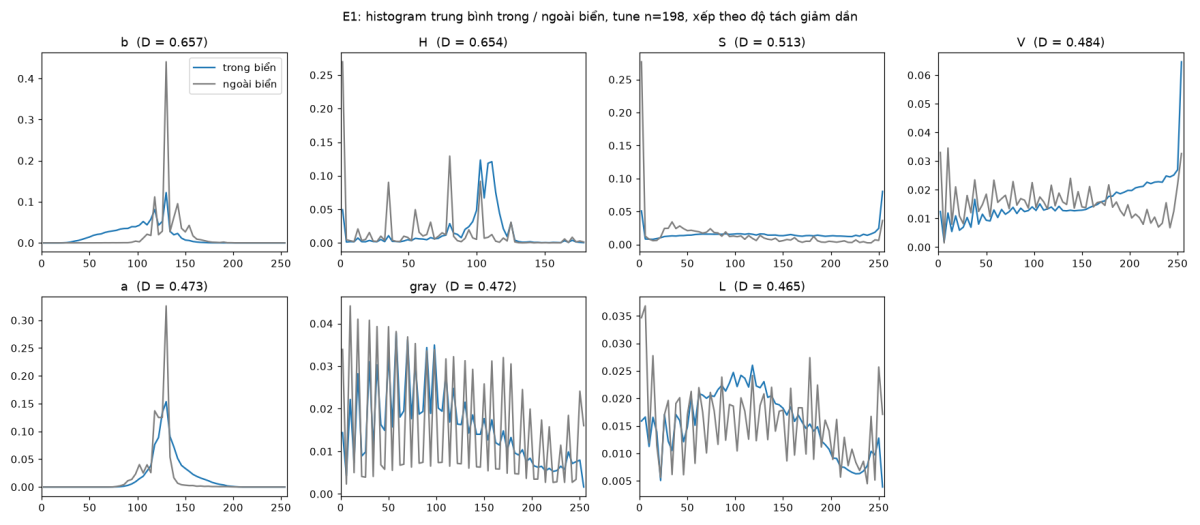
\includegraphics[width=\linewidth]{figures/e1_hist.png}\\[-1mm]
    {\footnotesize\color{muted} Xanh: trong biển, xám: ngoài biển. Hạng 3 kênh đầu không đổi với 32, 128 bin.}
    \vspace{1mm}

    {\small Định vị đang dùng ảnh xám. Ứng viên theo màu là hướng bổ sung (chưa thử), nhưng \hl{chỉ đúng với biển nền xanh}.}
  \end{columns}
\end{frame}

% ============ Định vị dựa biên + tinh chỉnh bộ lọc ============
\begin{frame}{Định vị dựa trên cạnh và tinh chỉnh bộ lọc ứng viên}
  \begin{columns}[T]
    \column{0.50\textwidth}
    \begin{enumerate}
      \item $|G_x|$ Sobel theo $x$, nhị phân Otsu.
      \item \emph{Close} ngang $21\times5$ nối nét ký tự, \emph{open} $3\times3$.
      \item \hl{Đa tỉ lệ}: thêm kernel $13\times3$ và $33\times7$, gộp bằng \hl{NMS} (IoU 0.5).
      \item Lọc theo \code{aspect}, \code{area\_ratio}, \code{fill\_ratio}, \code{edge\_density}, góc.
      \item Điểm heuristic, giữ top-5.
    \end{enumerate}
    \vspace{1mm}
    {\small \textbf{Tinh chỉnh bộ lọc}: nút thắt ở bộ lọc (tăng $k$ lên 10 không đổi). Sửa: hai kernel phụ, \code{area\_ratio} $[0.008,0.16]$, \code{aspect} $[1.5,7]$, chọn trên tune.}
    \column{0.48\textwidth}
    {\small\bfseries Trước và sau, tập test (\code{localize\_edge})}\\[1mm]
    \setlength{\tabcolsep}{3pt}\begin{tabularx}{\linewidth}{lCC}
      \rowcolor{accent}\hd{ALL ($n=462$)} & \hd{Cũ} & \hd{Chốt}\\
      Recall ứng viên (R@5) & 0.667 & \acc{0.792}\\
      \rowcolor{accentlight}Recall@1 (top-1) & 0.545 & \acc{0.682}\\
      Precision & 0.593 & \acc{0.729}\\
      \rowcolor{accentlight}Recall@1, nhóm \code{base} & 0.609 & \acc{0.751}\\
    \end{tabularx}
    \vspace{2mm}

    {\footnotesize Nhóm \code{db}, \code{challenge} gần như không đổi. Cái giá: thời gian tăng 40--50\% (đo khi máy tải, chỉ tương đối).}
  \end{columns}
\end{frame}

% ============ HOG + SVM + E3 ============
\begin{frame}{Xếp hạng lại bằng HOG + SVM (E3)}
  \begin{columns}[T]
    \column{0.33\textwidth}
    \begin{itemize}
      \item Crop bbox, resize $128\times32$, HOG 1620 chiều.
      \item \code{LinearSVC}, chỉ huấn luyện trên tune (198 dương, 594 âm).
      \item Chỉ xếp lại top-5, không thêm ứng viên.
      \item Top-1 test: \hl{0.682 $\to$ 0.751} (+32 ảnh).
      \item R@5 vẫn \hl{0.792}: trần xếp hạng.
    \end{itemize}
    \column{0.65\textwidth}
    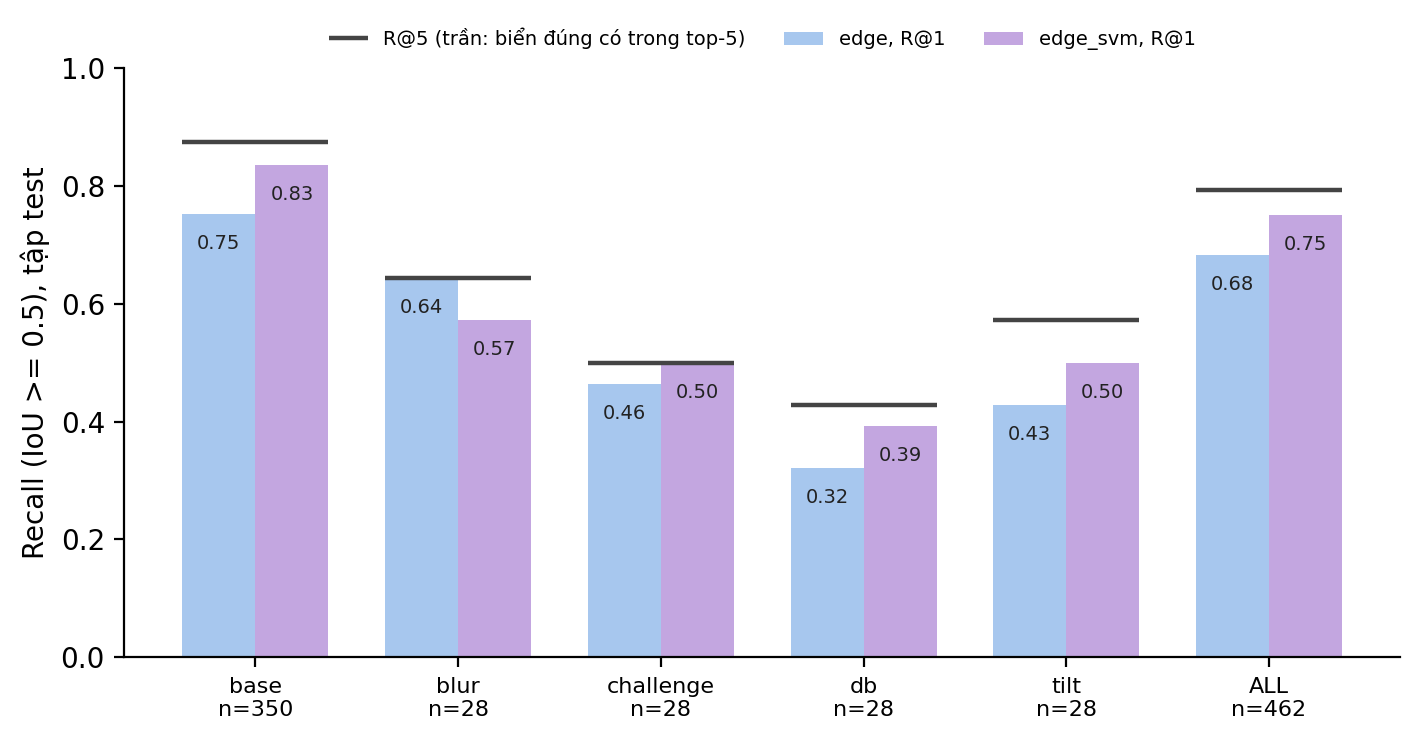
\includegraphics[width=\linewidth]{figures/e3_subset_r1.png}\\[-1mm]
    {\footnotesize\color{muted} Recall@1 theo nhóm (test), vạch đen là R@5. 21\% ảnh test không có ứng viên đúng trong top-5.}
  \end{columns}
\end{frame}

% ============ Nắn phối cảnh + E4 ============
\begin{frame}{Nắn phối cảnh và thí nghiệm E4: cắt bbox hay warp quad}
  \begin{columns}[T]
    \column{0.42\textwidth}
    \begin{itemize}
      \item Quad: mặt nạ xanh HSV + \code{approxPolyDP} (mặc định), lùi về \code{minAreaRect}.
      \item Homography đưa biển về $220\times70$.
      \item Đối chứng: cắt bbox ngang rồi resize.
      \item \code{tilt}: bbox không bù được nghiêng, \code{count\_match} 0.000 so với 0.429.
    \end{itemize}
    \column{0.56\textwidth}
    {\small\bfseries Tập test, toàn pipeline}\\[1mm]
    \small
    \setlength{\tabcolsep}{3pt}\begin{tabularx}{\linewidth}{lCC}
      \rowcolor{accent}\hd{Chỉ số} & \hd{bbox} & \hd{Quad}\\
      Sai số góc, tb (px), $n{=}347$ & 25.2 & \acc{16.3}\\
      \rowcolor{accentlight}Sai số góc, trung vị (px), $n{=}347$ & 19.4 & \acc{13.8}\\
      \code{all\_correct}, crop \code{gt}, $n{=}462$ & 0.262 & \acc{0.563}\\
      \rowcolor{accentlight}\code{all\_correct}, top-1 đúng, $n{=}347$ & 0.124 & \acc{0.259}\\
      Sai số góc \code{tilt} (px), $n{=}14$ & 68.0 & \acc{28.9}\\
    \end{tabularx}
    \vspace{2mm}

    {\footnotesize\color{muted} \code{blur} là ngoại lệ (16 ảnh, chênh 1--2 ảnh, chưa kết luận). \code{approxpoly} so với \code{minarearect}: khác biệt nhỏ, $p=0.46$.}
  \end{columns}
\end{frame}
% ============ Nhị phân hóa: phương pháp ============
\begin{frame}{Nhị phân hóa: Otsu và adaptive}
  \setbeamerfont{itemize/enumerate body}{size=\small}
  \begin{columns}[T]
    \column{0.49\textwidth}
    {\bfseries\color{accentdark}Otsu: một ngưỡng cho cả biển}
    \[t^{*}=\arg\max_{t}\;\omega_0\,\omega_1\,(\mu_0-\mu_1)^2\]
    {\small Cực đại phương sai giữa hai lớp (nền, chữ); hợp khi biển sáng đều, histogram hai đỉnh.}\\[3mm]
    {\bfseries\color{accentdark}Adaptive: ngưỡng riêng từng pixel}
    \[T(x,y)=m_G(x,y)-C,\quad 25\times25,\; C=7\]
    {\small $m_G$: trung bình Gauss quanh pixel. Chịu được bóng đổ, chói một bên.}
    \column{0.48\textwidth}
    \begin{block}{Lỗi gặp khi cài adaptive}
      \small Biển xanh chữ trắng: nền phẳng thành trắng, ký tự chỉ còn \hl{viền rỗng}.\\[1mm]
      Sửa: dùng Otsu để đoán cực tính (chữ sáng thì đảo ảnh), rồi \code{THRESH\_BINARY\_INV}. Có test đơn vị kiểm tra nền phẳng phải đen.
    \end{block}
    \vspace{2mm}
    \begin{itemize}
      \item Sau đó: đảm bảo chữ trắng (\code{ensure\_text\_white}), mở hình thái $2\times2$ xóa chấm nhiễu.
    \end{itemize}
  \end{columns}
\end{frame}

% ============ E5 kết quả ============
\begin{frame}{E5: Otsu và adaptive cho kết quả tương đương}
  \setbeamerfont{itemize/enumerate body}{size=\small}
  \begin{columns}[T]
    \column{0.45\textwidth}
    {\small\bfseries \code{all\_correct}, test, crop \code{gt}, CCA}\\[1mm]
    \small
    \setlength{\tabcolsep}{3pt}\begin{tabularx}{\linewidth}{lcCC}
      \rowcolor{accent}\hd{Nhóm} & \hd{$n$} & \hd{Otsu} & \hd{Adaptive}\\
      base & 350 & \textbf{0.666} & 0.611\\
      \rowcolor{accentlight}blur & 28 & \textbf{0.143} & 0.071\\
      challenge & 28 & 0.143 & \textbf{0.214}\\
      \rowcolor{accentlight}db & 28 & \textbf{0.393} & 0.250\\
      tilt & 28 & \textbf{0.286} & 0.214\\
      \rowcolor{accentlight}\textbf{ALL} & 462 & \textbf{0.563} & 0.509\\
    \end{tabularx}
    \begin{itemize}
      \item Theo cặp: 90 / 65 biển, $p\approx0.054$.
      \item Tune ngược lại (0.540 / 0.566) $\Rightarrow$ \hl{coi là hòa}, giữ Otsu.
    \end{itemize}
    \column{0.53\textwidth}
    \centering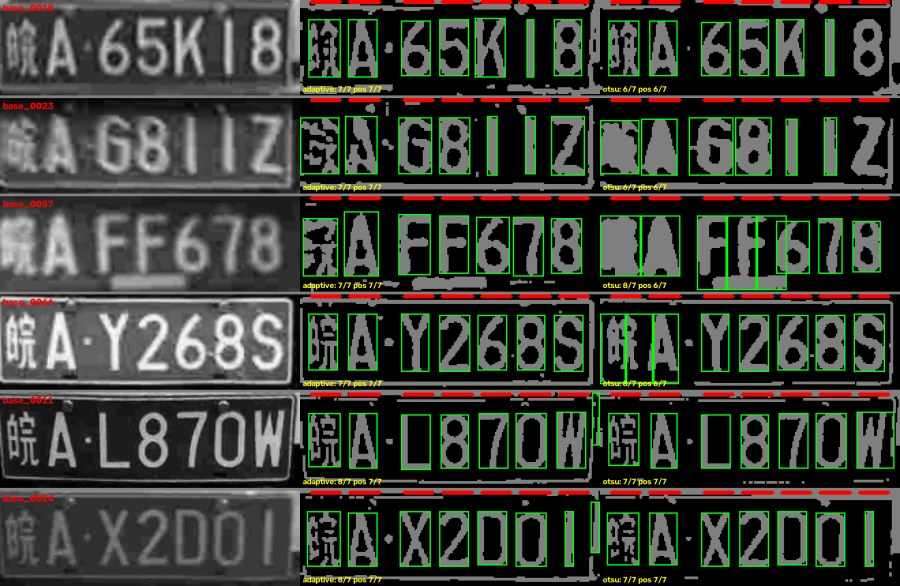
\includegraphics[width=\linewidth,height=0.5\textheight,keepaspectratio]{figures/e5_binarize.jpg}\\[-1mm]
    \raggedright
    {\footnotesize\color{muted} Ảnh gốc | adaptive | Otsu. Vạch đỏ: khuôn 7 vị trí.}
    \vspace{1mm}

    {\small \hl{Otsu hay làm dính} ký tự (148 biển $\le6$ hộp); \hl{adaptive hay thừa hộp} ở mép (85 biển $\ge8$ hộp).}
  \end{columns}
\end{frame}

% ============ Tách ký tự: phương pháp ============
\begin{frame}{Tách ký tự: CCA và projection}
  \begin{columns}[T]
    \column{0.49\textwidth}
    {\bfseries\color{accentdark}CCA (thành phần liên thông)}
    \begin{enumerate}
      \item Bỏ viền (rộng, rỗng), ốc vít (tâm lệch dọc). Khối rộng mà \emph{đặc} thì giữ lại để cắt.
      \item Gộp mảnh chồng nhau theo $x$ (ký tự Hán vỡ nét), gộp mảnh hẹp với mảnh kề.
      \item Lọc chiều cao, tỉ lệ, diện tích.
      \item Hộp rộng $\ge1.7\,w_{\mathrm{med}}$: \hl{cắt đều} thành $\mathrm{round}\big(\tfrac{w+g}{w_{\mathrm{med}}+g}\big)$ phần.
    \end{enumerate}
    \column{0.49\textwidth}
    {\bfseries\color{accentdark}Projection (chiếu theo cột)}
    \begin{enumerate}
      \item Bỏ viền, ốc vít như CCA; tách dòng bằng chiếu ngang.
      \item Profile cột: cột có $\ge10\%$ chiều cao là trắng thì là cột chữ.
      \item Nối dải gần nhau, bỏ dải quá hẹp.
      \item Dải rộng: \hl{cắt tại thung lũng} (cột ít trắng nhất) quanh vị trí dự kiến.
    \end{enumerate}
  \end{columns}
  \vspace{2mm}
  {\small\color{muted} Mọi ngưỡng tính theo tỉ lệ kích thước biển; tham số thí nghiệm lấy từ config.}
\end{frame}

% ============ Tinh chỉnh trên tune ============
\begin{frame}{Tinh chỉnh trên tune: sửa độ đo cho chữ số ``1''}
  \begin{columns}[T]
    \column{0.44\textwidth}
    \begin{itemize}
      \item Số ``1'' rộng $\approx$ 9 px, khuôn 22.5 px $\Rightarrow$ IoU $\approx0.4$ dù nằm đúng giữa khuôn.
      \item Trước khi sửa: chỉ \hl{3/56} vị trí ``1'' được tính đúng, so với 889/994 ký tự khác.
      \item Luật tâm: hộp hẹp ($\le0.6\times$ khuôn) trúng nếu \hl{tâm nằm trong khuôn}.
      \item Bản chốt: ngưỡng mảnh hẹp riêng, cắt có tính khe, lọc mảnh dẹt sau khi gộp.
    \end{itemize}
    \column{0.54\textwidth}
    {\small\bfseries \code{all\_correct}, tune $n=198$, crop \code{gt}}\\[1mm]
    \small
    \setlength{\tabcolsep}{3pt}\begin{tabularx}{\linewidth}{YCC}
      \rowcolor{accent}\hd{Phiên bản} & \hd{Otsu+CCA} & \hd{Otsu+proj.}\\
      Bản đầu & 0.338 & --\\
      \rowcolor{accentlight}Giữ khối đặc để cắt & 0.364 & --\\
      Luật tâm cho ``1'' & 0.515 & 0.566\\
      \rowcolor{accentlight}\textbf{Bản chốt} & 0.540 & \acc{0.596}\\
    \end{tabularx}
    \vspace{2mm}

    {\footnotesize\color{muted} Mỗi bước xuất phát từ đọc ảnh lỗi, không quét lưới. Hằng số chọn trên chính tune nên số tune hơi lạc quan.}
  \end{columns}
\end{frame}

% ============ E6 ============
\begin{frame}{E6: projection tốt hơn CCA, ổn định trên cả hai tập}
  \setbeamerfont{itemize/enumerate body}{size=\small}
  \begin{columns}[T]
    \column{0.47\textwidth}
    {\small\bfseries Test, Otsu, \code{all\_correct}}\\[1mm]
    \small
    \setlength{\tabcolsep}{2.5pt}\begin{tabularx}{\linewidth}{lCCCC}
      \rowcolor{accent}\hd{Nhóm} & \hd{CCA gt} & \hd{proj. gt} & \hd{CCA pred} & \hd{proj. pred}\\
      base & 0.666 & \textbf{0.749} & 0.243 & \textbf{0.277}\\
      \rowcolor{accentlight}blur & 0.143 & \textbf{0.214} & 0.000 & \textbf{0.071}\\
      challenge & 0.143 & \textbf{0.214} & \textbf{0.071} & 0.000\\
      \rowcolor{accentlight}db & \textbf{0.393} & 0.250 & \textbf{0.107} & 0.071\\
      tilt & 0.286 & 0.286 & 0.000 & 0.000\\
      \rowcolor{accentlight}\textbf{ALL} & 0.563 & \acc{0.626} & 0.195 & \acc{0.219}\\
    \end{tabularx}
    \vspace{1mm}
    \begin{itemize}
      \item Theo cặp: 47 / 18 biển, \hl{$p<0.001$}; tune cùng chiều.
      \item Ít thiếu hộp hơn: 148 $\to$ 110 biển.
    \end{itemize}
    \column{0.51\textwidth}
    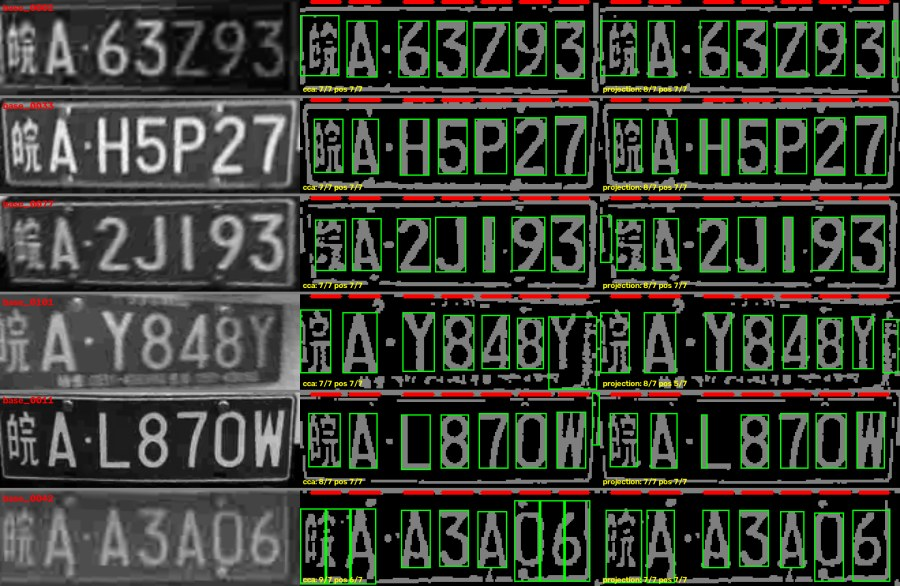
\includegraphics[width=\linewidth]{figures/e6_segment.jpg}\\[-1mm]
    {\footnotesize\color{muted} Ảnh gốc | CCA | projection. CCA cắt đều khối ``06'' dính nhiễu thành 3 hộp; projection không bị nhưng hay thừa hộp ở mép, và cắt ``H'' thành hai nét.}
  \end{columns}
\end{frame}
% ============ E7 thời gian ============
\begin{frame}{Thời gian chạy từng bước (E7)}
  \begin{columns}[T]
    \column{0.58\textwidth}
    {\small\bfseries ms/ảnh, trung bình, tập test, một tiến trình}\\[2mm]
    \begin{tikzpicture}[xshift=9mm,x=0.040cm,y=0.9cm,font=\small]
      \barrow{3.0}{Tiền xử lý}{69.79}{69.8}
      \barrow{2.0}{Sobel, morph, lọc, NMS}{63.50}{63.5}
      \barrow{1.0}{HOG + SVM}{4.77}{4.8}
      \barrow{0.0}{Nắn, nhị phân, tách}{1.84}{1.8}
    \end{tikzpicture}
    \column{0.40\textwidth}
    \begin{itemize}
      \item Tổng \hl{139.8 ms/ảnh} (p95 262.2 ms).
      \item Định vị chiếm gần hết: tiền xử lý $\approx$ 50\% (chủ yếu bilateral), Sobel + morph $\approx$ 45\%, SVM $\approx$ 3\%.
      \item Nắn, nhị phân hóa, tách ký tự cộng lại chỉ 1.8 ms.
    \end{itemize}
  \end{columns}
  \vspace{1mm}
  \begin{block}{Lưu ý khi đọc số}
    \small Đo trên máy ít tải nhưng không phải máy chuyên dụng; lần ghi trong sổ thí nghiệm là 416 ms/ảnh (máy đang chạy nhiều tiến trình). Chỉ nên đọc tỉ lệ tương đối giữa các bước.
  \end{block}
\end{frame}
% ============ E8 ============
\begin{frame}{E8: biển Việt Nam, kết quả chính}
  \setbeamerfont{itemize/enumerate body}{size=\small}
  \begin{columns}[T]
    \column{0.47\textwidth}
    \begin{itemize}
      \item 187 ảnh (Kaggle 75 + 64, Brave 48); chạy trên 139 ảnh Kaggle có bbox, chỉ xem bằng mắt.
      \item Định vị đạt \hl{40/139}; tách đạt 33 (crop \code{gt}) và 22 (crop \code{pred}).
      \item Biển 1 dòng ($n=44$): định vị 28, tách (\code{gt}) 30.
      \item Biển 2 dòng ($n=95$): định vị 12, tách (\code{gt}) \hl{3}.
    \end{itemize}
    \column{0.51\textwidth}
    \centering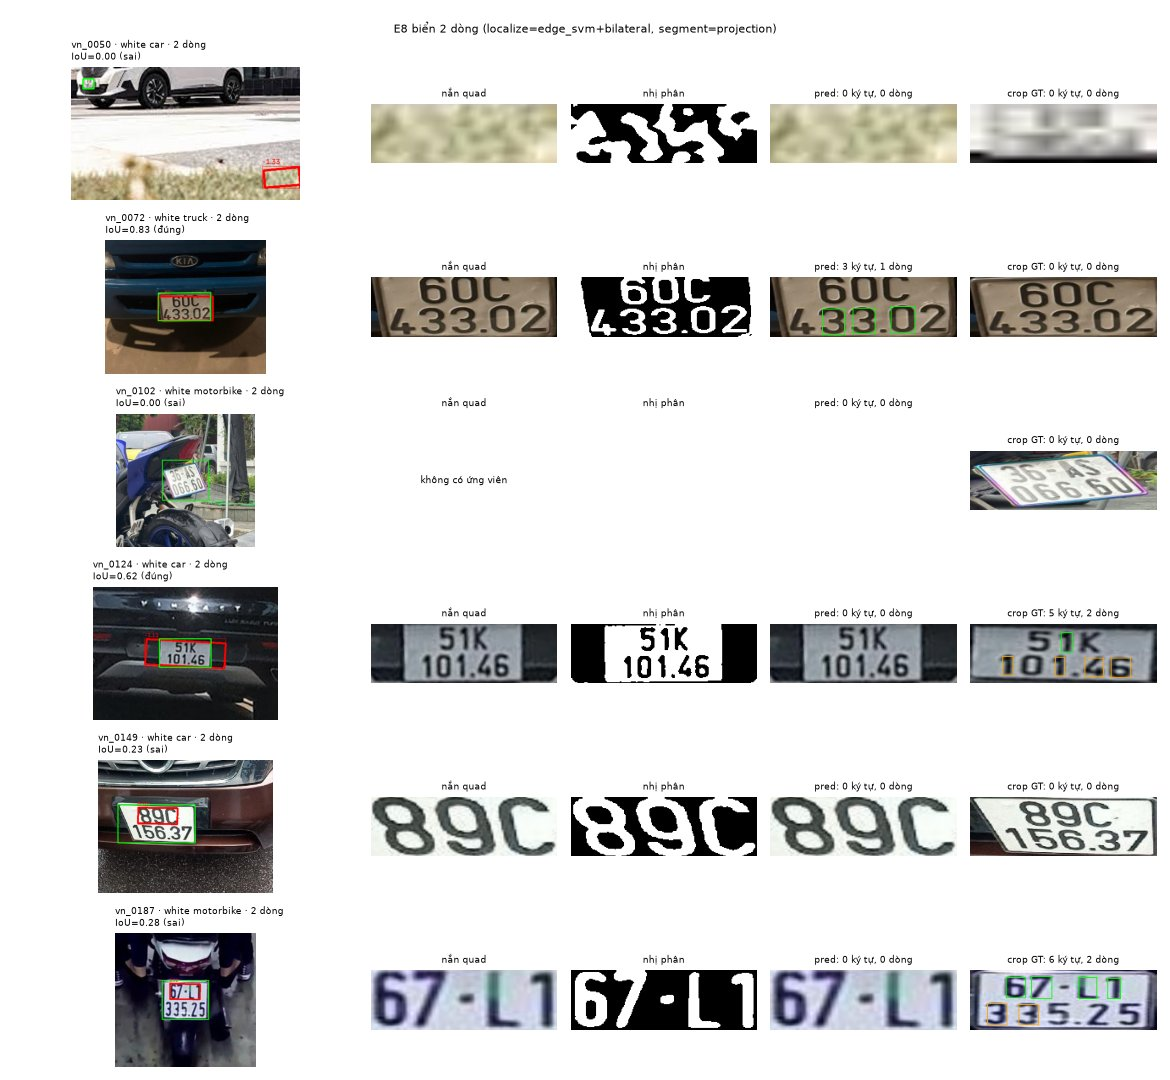
\includegraphics[width=\linewidth,height=0.62\textheight,keepaspectratio]{figures/vn_two_line.jpg}\\[-1mm]
    {\footnotesize\color{muted} Biển 2 dòng: chỉ \code{vn\_0072}, \code{0124} định vị đúng, vẫn tách 0--3 hộp; 4 ảnh còn lại sai hoặc không có ứng viên.}
  \end{columns}
\end{frame}

\begin{frame}{E8: nơi pipeline hỏng trên biển Việt Nam}
  \setbeamerfont{itemize/enumerate body}{size=\small}
  \begin{columns}[T]
    \column{0.45\textwidth}
    \centering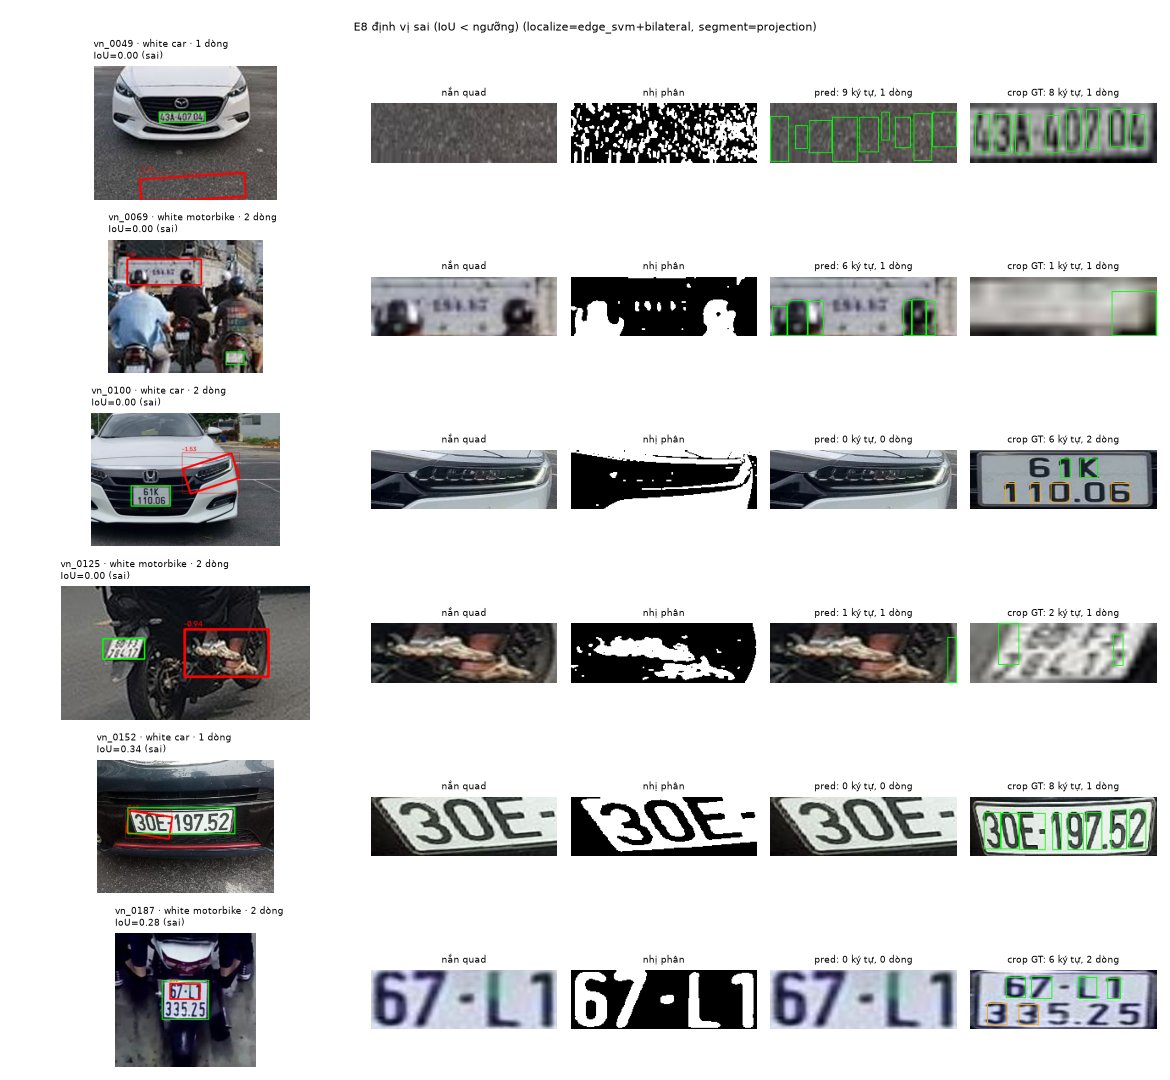
\includegraphics[width=\linewidth,height=0.62\textheight,keepaspectratio]{figures/vn_loc_fail.jpg}\\[-1mm]
    {\footnotesize\color{muted} Định vị sai: mặt đường, đèn, chân, biển/chữ khác trong ảnh đông xe; có hộp chỉ phủ một phần biển.}
    \column{0.53\textwidth}
    \begin{itemize}
      \item Xe máy: định vị 2/61 (tất cả biển 2 dòng). Ô tô 34/66.
      \item Biển vàng (6 ảnh) không ảnh nào đạt; biển xanh, đỏ chỉ 1 ảnh mỗi loại: chỉ là giai thoại.
      \item Biển 2 dòng bị nắn $220\times70$ và \code{split\_lines} chỉnh trên CCPD (giả thuyết, chưa tách riêng).
    \end{itemize}
  \end{columns}
\end{frame}

% ============ Triage ============
\begin{frame}{Triage lỗi: mỗi ảnh test mất ở bước nào?}
  \begin{columns}[T]
    \column{0.62\textwidth}
    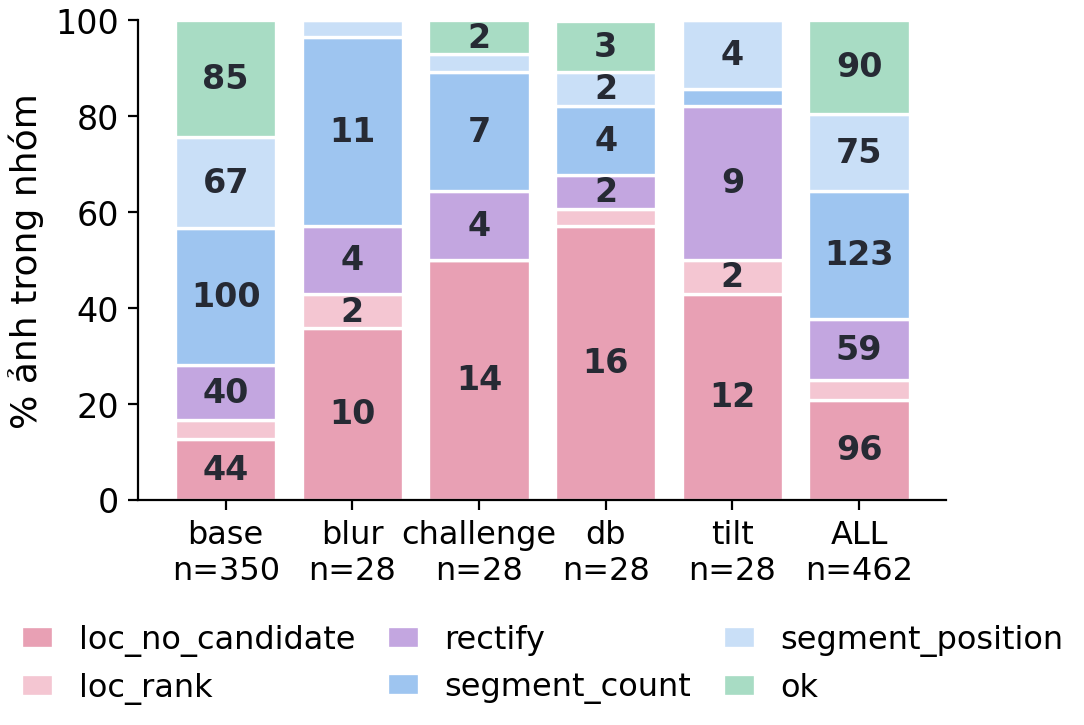
\includegraphics[width=\linewidth,height=0.66\textheight,keepaspectratio]{figures/triage_stages_slide.png}
    \column{0.36\textwidth}
    \footnotesize
    \setlength{\tabcolsep}{2pt}
    \begin{tabularx}{\linewidth}{>{\raggedright\arraybackslash}Xrr}
      \rowcolor{accent}\hd{Bước lỗi chính} & \hd{Ảnh} & \hd{\%\,}\\
      \code{loc\_no\_candidate} & 96 & 20.8\\
      \rowcolor{accentlight}\code{loc\_rank} & 19 & 4.1\\
      \code{rectify} & 59 & 12.8\\
      \rowcolor{accentlight}\code{segment\_count} & 123 & 26.6\\
      \code{segment\_position} & 75 & 16.2\\
      \rowcolor{accentlight}\code{ok} & \textbf{90} & \textbf{19.5}\\
    \end{tabularx}
    \vspace{2mm}

    {\footnotesize Mỗi ảnh một bước lỗi chính, xét theo thứ tự pipeline. Nhóm khó gần như không có ảnh \code{ok} (0--3 trên 28).}
  \end{columns}
\end{frame}

% ============ Phát hiện chính ============
\begin{frame}{Phát hiện chính từ phân tích lỗi}
  \begin{columns}[T]
    \column{0.62\textwidth}
    \begin{itemize}
      \item \hl{Định vị mất ở khâu sinh ứng viên}: 96 ảnh \code{loc\_no\_candidate} so với 19 ảnh \code{loc\_rank}; chỉ 12/96 do bbox nhỏ hơn cận diện tích.
      \item \hl{Xếp hạng}: 18/19 ảnh có biển đúng ở hạng 2; top-1 thường là logo hoặc chữ hãng xe.
      \item \hl{Crop dự đoán và bộ tách cùng bậc}: trong 257 ảnh top-1 đúng nhưng vẫn lỗi, \acc{152} tách đúng ở crop \code{gt} (lỗi do crop dự đoán), \acc{105} tách sai cả ở crop \code{gt} (lỗi do bộ tách).
      \item 54/123 ảnh \code{segment\_count} có 6 hộp do ký tự Hán dính chữ A.
    \end{itemize}
    \column{0.34\textwidth}
    \centering
    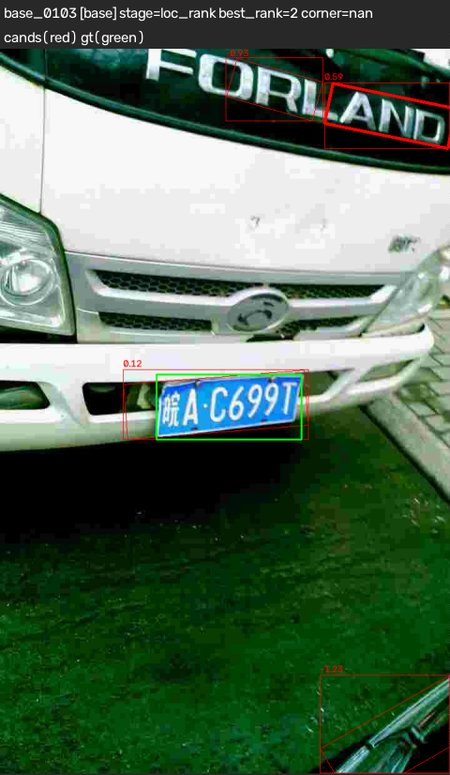
\includegraphics[height=0.58\textheight]{figures/loc_rank_cands.png}\\[-1mm]
    {\footnotesize\color{muted} \code{loc\_rank}: ứng viên đỏ, bbox thật xanh. Top-1 là chữ hãng xe, biển thật ở hạng 2.}
  \end{columns}
\end{frame}

% ============ gt -> pred ============
\begin{frame}{Lỗi tổng thể chủ yếu nằm trước bước tách}
  \setbeamerfont{itemize/enumerate body}{size=\small}
  \begin{columns}[T]
    \column{0.52\textwidth}
    \begin{tikzpicture}[x=4.8cm,y=0.75cm,font=\small]
      \foreach \y/\lab/\v/\t in {3/{proj., crop \code{gt}}/0.626/0.626, 2/{CCA, crop \code{gt}}/0.563/0.563, 1/{proj., crop \code{pred}}/0.219/0.219, 0/{CCA, crop \code{pred}}/0.195/0.195}{
        \node[anchor=east] at (-0.03,\y) {\lab};
        \fill[accent] (0,\y-0.27) rectangle (\v,\y+0.27);
        \node[anchor=west] at (\v+0.02,\y) {\t};
      }
    \end{tikzpicture}\\[1mm]
    {\footnotesize\color{muted} \code{all\_correct} trên test, $n=462$.}
    \column{0.46\textwidth}
    \begin{itemize}
      \item \hl{0.626 $\to$ 0.219} khi thay quad thật bằng quad dự đoán.
      \item 25\% ảnh định vị sai; quad dự đoán lệch trung bình 16 px (E4).
      \item Triage: 64/123 ảnh \code{segment\_count} tách đúng nếu crop bằng quad thật.
      \item Lỗi của chính bộ tách: ký tự Hán \hl{dính chữ ``A''} (6 hộp) và mảnh viền ở mép (8 hộp).
    \end{itemize}
  \end{columns}
  \vspace{1mm}
  \begin{block}{Đánh giá theo hộp gán tay (30 biển test, 210 hộp)}
    \small CCA: P 0.945, R 0.819, F1 0.878 \quad|\quad projection: P 0.962, R 0.838, \hl{F1 0.896} (base: 0.977). P cao hơn R: hộp sinh ra thường ôm đúng ký tự, lỗi chủ yếu là \emph{thiếu} hộp.
  \end{block}
\end{frame}

% ============ Hạn chế ============
\begin{frame}{Hạn chế và hướng cải thiện}
  \setbeamerfont{itemize/enumerate body}{size=\footnotesize}
  \begin{columns}[T]
    \column{0.50\textwidth}
    {\bfseries\color{accentdark}Hạn chế}
    \begin{itemize}
      \item IoU trục ngang phạt biển nghiêng.
      \item Nhóm khó chỉ 28 ảnh test (một ảnh = 0.036), chưa có khoảng tin cậy, một lần chia tune/test.
      \item CV của SVM chia theo patch nên lạc quan.
      \item Chọn \code{approxpoly} dựa trên 128 ảnh tune, ngưỡng triage trên 50 ảnh.
      \item Hằng số tách ký tự chọn trên tune; khuôn lệch $\approx$ 3 px; hộp gán tay chỉ 30 biển.
      \item Thời gian đo trên máy không chuyên dụng.
      \item E8 chỉ định tính: 139 ảnh, nhỏ và không cân bằng (1 xanh, 1 đỏ, 6 vàng); 48 ảnh crawl chưa gán nhãn.
    \end{itemize}
    \column{0.48\textwidth}
    {\bfseries\color{accentdark}Hướng cải thiện}
    \begin{itemize}
      \item Thêm nguồn ứng viên theo \hl{màu biển} (E1) hoặc bù nghiêng trước morph (chưa thử); 21\% ảnh không có ứng viên đúng.
      \item SVM: thêm \hl{mẫu âm khó} (logo, chữ hãng xe), chia fold theo ảnh.
      \item Nắn: quad chính xác hơn (sai số $\approx$ 16 px); nắn theo tỉ lệ biển 2 dòng.
      \item \hl{Projection} làm mặc định; xử lý ký tự Hán dính ``A''.
      \item Đánh giá bằng \hl{IoU đa giác}; gán bbox cho 48 ảnh Brave.
    \end{itemize}
  \end{columns}
\end{frame}

% ============ Kết luận ============
\begin{frame}{Kết luận}
  \begin{itemize}
    \item Pipeline cổ điển trên CCPD: định vị \code{edge\_svm} top-1 đúng \acc{75.1\%}, nắn quad, tách projection.
    \item Trên crop thật, bộ tách đúng hết \acc{62.6\%} biển; toàn pipeline chỉ \acc{19.5--21.9\%}.
    \item Nút thắt theo thứ tự ưu tiên:
    \begin{enumerate}
      \item \hl{Sinh ứng viên}: 21\% ảnh không có ứng viên đúng trong top-5 $\to$ thêm ứng viên theo màu, mẫu âm khó cho SVM.
      \item \hl{Nắn}: quad lệch $\approx$ 16 px làm hỏng crop.
      \item \hl{Tách}: ký tự Hán dính ``A'', mảnh viền ở mép.
    \end{enumerate}
    \item Mọi lựa chọn làm trên CCPD (nền xanh, 1 dòng, 7 ký tự); trên 139 ảnh biển VN (E8), định vị đạt 40; khá với ô tô 1 dòng, kém với biển 2 dòng và xe máy.
  \end{itemize}
\end{frame}

% ============ Cảm ơn ============
\begin{frame}[plain]
  \begin{tikzpicture}[remember picture,overlay]
    \fill[accent] (current page.south west) rectangle (current page.north east);
    \node[text=white,align=center,text width=0.8\paperwidth] at (current page.center)
      {{\fontsize{28}{32}\selectfont\bfseries Cảm ơn thầy và các bạn đã lắng nghe}\\[6mm]
       {\large Xin mời thầy và các bạn đặt câu hỏi}};
  \end{tikzpicture}
\end{frame}

\end{document}
